\documentclass[12pt,a4paper]{article}
\usepackage{amsmath}
\usepackage{amsfonts}
\usepackage{amssymb}
\usepackage{graphicx}
\usepackage{secdot}
\usepackage[left=2cm,right=2cm,top=2cm,bottom=2cm]{geometry}

\title{Experiment- 1}
\author{Shibayan Biswas, AE21B109\\ Department of Aerospace Engineering\\ IIT Madras\\[3ex] Instructor:\\ \large Professor Dr. Manikandan Mathur}

\date{September 12, 2022}


\begin{document}
\maketitle
\hline


\section{Aim:}
To investigate the validity of the Bernoulli's equation when it is applied to a steady flow of air through Subsonic Wind Tunnel. 
\section{Introduction:}
Energy presents in the form of pressure, velocity, and elevation in fluids with no energy exchange due to viscous dissipation, heat transfer, or shaft work (pump or some other device). The relationship among these three forms of energy was first stated by Daniel Bernoulli (1700-1782), based upon the conservation of energy principle. Bernoulli’s theorem pertaining to a flow streamline is based on three assumptions: steady flow, in-compressible fluid, and no losses from the fluid friction. The validity of Bernoulli’s equation will be examined in this experiment.
\section{Practical Application:}
Bernoulli’s theorem provides a mathematical means to understanding the mechanics of fluids. It has many real-world applications, ranging from understanding the aerodynamics of an airplane; calculating wind load on buildings; designing water supply and sewer networks; measuring flow using devices such as weirs, Parshall flumes, and venturimeters; and estimating seepage through soil, etc. Although the expression for Bernoulli’s theorem is simple, the principle involved in the equation plays vital roles in the technological advancements designed to improve the quality of human life.
\section{Objective:}
The objective of this experiment is to investigate the validity of the Bernoulli equation when it is applied to a steady flow of water through a tapered duct.
\section{Equipment:}
The following equipment is required to complete the demonstration of the Bernoulli equation experiment:
\begin{itemize}
\item Subsonic Wind Tunnel(Should have a honey comb structure to ensure steady flow and a blower to suck the air from the tunnel)
\item Pitot Tube 
\item Computer(Software installed for passing values as input and getting the corresponding values as output)
\end{itemize}
\begin{figure}[!ht]
	\begin{center}
		\framebox{
			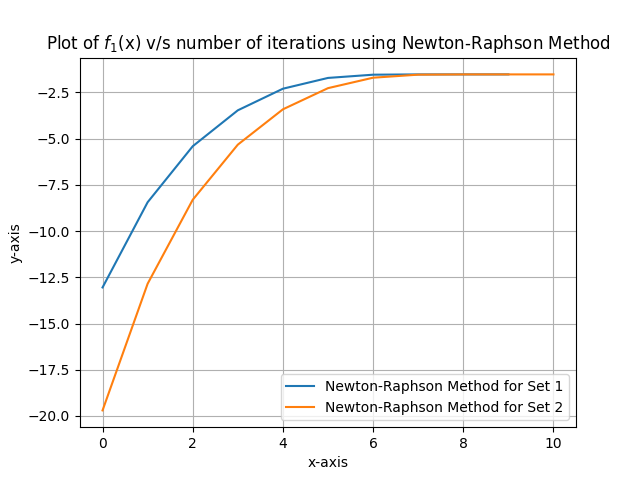
\includegraphics[scale=0.4]{Figure_3.png}
		}
	\end{center}
	\caption{MP 315D Subsonic Wind Tunnel}
\end{figure}
\clearpage
\begin{figure}[!ht]
	\begin{center}
		\framebox{
			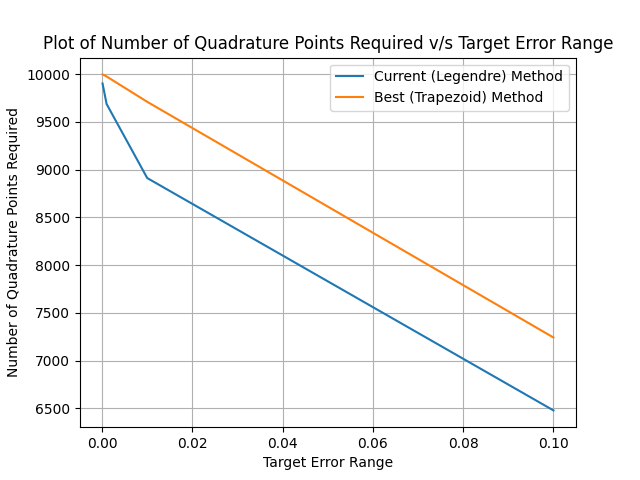
\includegraphics[scale=0.55]{Figure_4.png}
		}
	\end{center}
	\caption{Complete Experimental Setup}
\end{figure}
\section{Theory:}


Bernoulli’s theorem, in fluid dynamics,is relation among the pressure, velocity, and elevation in a moving fluid (liquid or gas), the compressibility and viscosity (internal friction) of which are negligible and the flow of which is steady, or laminar. First derived (1738) by the Swiss mathematician Daniel Bernoulli, the theorem states, in effect, that the total mechanical energy of the flowing fluid, comprising the energy associated with fluid pressure, the gravitational potential energy of elevation, and the kinetic energy of fluid motion, remains constant. Bernoulli’s theorem is the principle of energy conservation for ideal fluids in steady, or streamline, flow and is the basis for many engineering applications.\\
\\In most flows of liquids, and of gases at low Mach number, the density of a fluid parcel can be considered to be constant, regardless of pressure variations in the flow.These flows are called in-compressible flows. Bernoulli performed his experiments on liquids, so his equation in its original form is valid only for in-compressible flow. A common form of Bernoulli’s equation is:\\
\begin{equation}
\frac{p}{\rho} + \frac{v^2}{2} + \text{gz} = constant
\end{equation}
P: pressure\\
z: height of the fluid\\
$\rho$ : density of liquid\\
v: fluid velocity\\
g: acceleration\\
due to gravity\\
\\In Bernoulli’s hypothesis the stream is friction-less, consistent, and in-compressible. These presumptions are additionally founded on the laws of conservation of mass and energy. Subsequently, the initial mass and energy for a given control volume are equivalent to the final mass and energy:\\
\begin{equation}
Q_{in} = Q_{out}
\end{equation}
\begin{equation}
E_{in} = E_{out}
\end{equation}
In this experiment,the duct is horizontal,so the difference in height can be
neglected,it implies $z_1=z_2$.\\
The hydrostatic pressure (P) along the flow is measured, and the pressure
head (h), is:
\begin{equation}
\text{h} = \frac{p}{\text{$\rho$g}}
\end{equation}
Therefore, Bernoulli’s equation for the test section can be written as:
\begin{equation}
h_1 + \frac{v_1^2}{2g} = h_2 + \frac{v_2^2}{2g}
\end{equation}
in which $\frac{v^2}{2g}$ is called the velocity head ($h_d$)\\
The total head might be estimated by the crossing hypodermic test. This
test is embedded into the channel with its end-opening confronting the
stream so the stream becomes stale locally at this end; thus:
The total head might be estimated by the crossing hypodermic test. This test is embedded into the channel with its end-opening confronting the stream so the stream becomes stale locally at this end; thus:
\begin{equation}
h_t  = h + \frac{v^2}{2g}
\end{equation}
The conservation of energy can be expressed as:
\begin{equation}
h_{t1}  = h_{t2} 
\end{equation}
The flow velocity is measured by dividing volume of the fluid (V) that passes over a time period (t). The flow rate is measured as:
\begin{equation}
Q  = \frac{V}{t}
\end{equation}
The velocity of flow at any section of the duct with a cross-sectional area is:
\begin{equation}
v  = \frac{Q}{A}
\end{equation}
For an in-compressible fluid, conservation of mass(Equation 2) can be applied across the test section since mass is not accumulating,that implies:
\begin{equation}
A_1 v_1  = A_1 v_1
\end{equation}
\section{Procedure:}
In this experiment, the validity of Bernoulli’s equation is determined with the help of a subsonic wind tunnel which measure the pressure head and total head at certain points along the flow.
\begin{itemize}
\item Setting up the wind tunnel.
\item Turning on the fan of wind tunnel.
\item Setting the speed of the fan to certain value,which gives us corresponding wind velocity.
\item Note down the pressure readings of the 11 ports which are displayed on computer.
\item Now changing the fan speed and repeat the experiment until you get 3 such readings.
\item We can note the static pressure as shown on the screen,and use Bernoulli’s equation to figure out pressure at every one of those 11 ports and later check results between theoretical and experimental values.
\end{itemize}
\begin{figure}[!ht]
	\begin{center}
			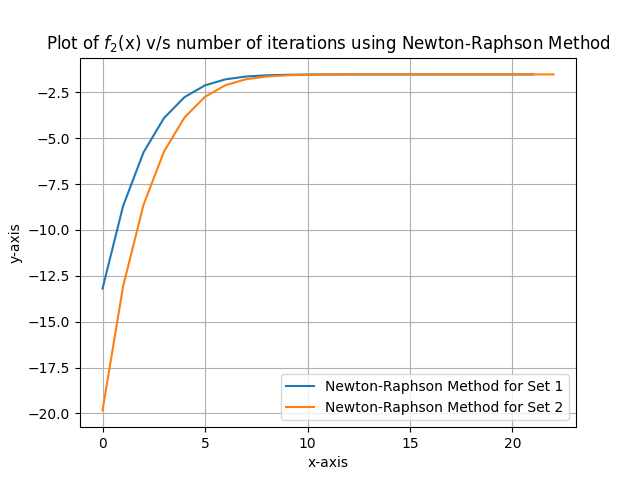
\includegraphics[scale=0.25]{Figure_6.png}
	\end{center}
	\caption{Working of a Subsonic Wind Tunnel}
\end{figure}
\section{Results:}
The tables representing the experimental and the theoretical values along with the plots showing the variation of the respective values for the following experiment is provided in this section:
\begin{itemize}
\item For velocity of wind v = 12.4 m/s at pressure P = 9.0 mm of water, the following is the pressure and velocity distribution at distribution cross sections of the test section.
\clearpage
\begin{table}
\begin{center}
\begin{tabular}{|p{5cm}|p{3cm}|p{2.5cm}|p{2.5cm}|p{2.5cm}|}
\hline
Static Pressure(Pa) & Area($mm^2$) & Velocity(m/s) & $\frac{1}{2} \rho v^2$ & P + $\frac{1}{2} \rho v^2$ \\ 
\hline
88.29&22350&12.4&94.18&182.47\\
105.95&19860&13.95&119.19&225.14\\
143.23&17370&15.96&156.02&299.25\\
109.97&15000&18.48&209.18&319.05\\
186.39&15000&18.48&209.18&395.57\\
128.51&15000&18.48&209.18&337.67\\
169.71&16395&16.90&174.94&344.65\\
133.42&17902.5&15.48&146.77&280.19\\
132.44&19410&14.28&124.9&257.34\\
119.68&20910&13.25&107.53&227.21\\
112.82&22410&12.37&93.72&206.54\\
\hline
\end{tabular}
\end{center}
\end{table}
\begin{figure}[!ht]
	\begin{center}
			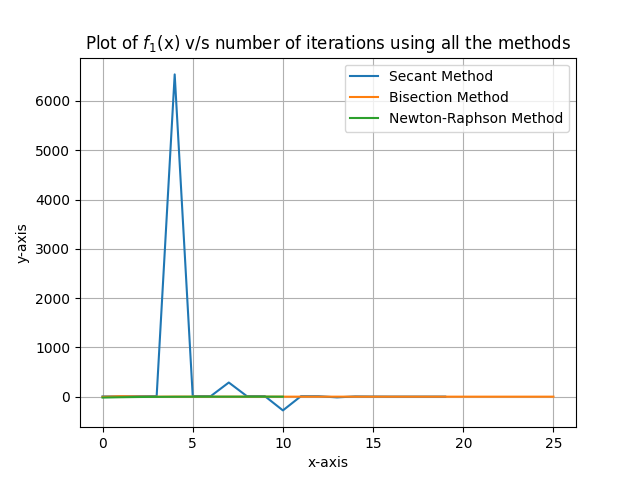
\includegraphics[scale=0.45]{Figure_7.png}
	\end{center}
	\caption{P + $\text{$\frac{1}{2} \rho v^2$}$ v/s P}
\end{figure}
\item For velocity of wind v = 17.5 m/s at pressure P = 17.9 mm of water, the following is the pressure and velocity distribution at distribution cross sections of the test section.
\clearpage
\begin{table}
\begin{center}
\begin{tabular}{|p{5cm}|p{3cm}|p{2.5cm}|p{2.5cm}|p{2.5cm}|}
\hline
Static Pressure(Pa) & Area($mm^2$) & Velocity(m/s) & $\frac{1}{2} \rho v^2$ & P + $\frac{1}{2} \rho v^2$ \\ 
\hline
175.6&22350&17.5&187.58&363.18\\
206.99&19860&19.69&237.46&444.45\\
236.42&17370&22.52&310.63&547.05\\
217.78&15000&26.08&416.6&634.38\\
368.87&15000&26.08&416.6&785.47\\
255.06&15000&26.08&416.6&671.66\\
333.54&16395&23.86&348.70&682.24\\
272.72&17902.5&21.85&292.42&565.14\\
268.79&19410&20.15&248.69&517.48\\
235.44&20910&18.71&214.41&449.85\\
218.76&22410&17.45&186.51&405.27\\
\hline
\end{tabular}
\end{center}
\end{table}
\begin{figure}[!ht]
	\begin{center}
			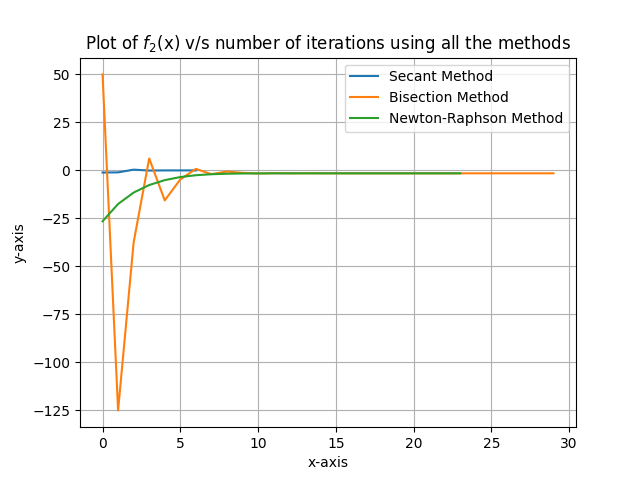
\includegraphics[scale=0.55]{Figure_8.png}
	\end{center}
	\caption{P + $\frac{1}{2} \rho v^2$ v/s P}
\end{figure}
\item For velocity of wind v = 22.2 m/s at pressure P = 28.6 mm of water, the following is the pressure and velocity distribution at distribution cross sections of the test section.
\clearpage
\begin{table}
\begin{center}
\begin{tabular}{|p{5cm}|p{3cm}|p{2.5cm}|p{2.5cm}|p{2.5cm}|}
\hline
Static Pressure(Pa) & Area($mm^2$) & Velocity(m/s) & $\text{$\frac{1}{2} \rho v^2$}$ & P + $\text{$\frac{1}{2} \rho v^2$}$ \\ 
\hline
280.57 &22350 &22.2 &301.86 &582.43\\
335.5 &19860 &24.98 &382.2 &717.7\\
363.95 &17370 &28.56 &499.6 &863.55\\
355.12 &15000 &33.08 &670.25 &1025.37\\
594.49 &15000 &33.08 &670.25 &1264.74\\
413 &15000 &33.08 &670.25 &1083.25\\
534.65 &16395 &30.26 &560.85 &1095.5\\
438.51 &17902.5 &27.72 &470.64 &909.15\\
428.7 &19410 &25.56 &400.15 &828.85\\
377.69 &20910 &23.73 &344.91 &722.6\\
352.18 &22410 &22.14 &300.24 &652.42\\
\hline
\end{tabular}
\end{center}
\end{table}
\begin{figure}[!ht]
	\begin{center}
			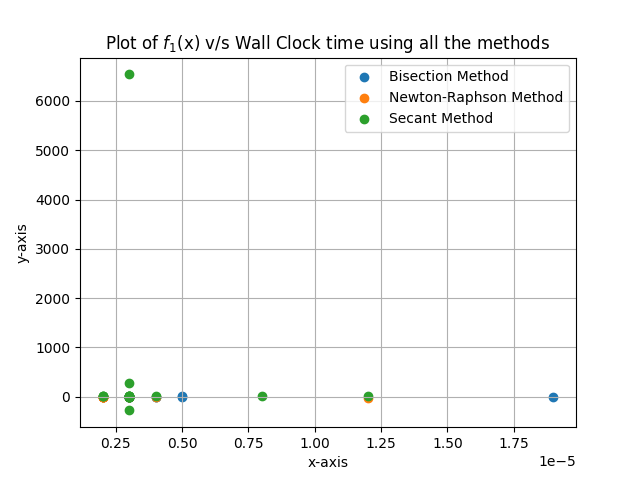
\includegraphics[scale=0.95]{Figure_9.png}
	\end{center}
	\caption{P + $\frac{1}{2} \rho v^2$ v/s P}
\end{figure}
\end{itemize}
\section{Interpretation:}
The graphs of experimental and theoretical pressure variations have a lot of differences because the conditions we assumed are not ideally present, and there are many errors such as equip-mental errors,variation of temperature,variation of atmospheric pressure,variation in the flow of wind i.e not perfectly steam line etc...But the over all idea of the graphs are same i.e graph decreases until certain value and then increases.So we can conclude that Bernoulli’s equation is valid.
\section{Sources of Error:}
While playing out the experiments, there are some mistakes noticed.. may be it’s little relying upon the precision with which we are playing out the analysis however there’s mistake certainly. Given beneath are a few potential causes of blunder while playing out this experiments:
\begin{itemize}
\item Error in Instruments- Equipment used in the experiments are man made and bound to have certain errors.
\item Improper conditions-T he conditions at the time of experiment might be off without our notice which ultimately lead to errors.
\item Human error- Everything humans do isn’t perfects and often challenged to have some mistakes.
\item Parallax error- The apparent shift in an object’s position as it is viewed from different angles is one of the errors we face.
\end{itemize}
\section{Conclusion:}
Even though barring minor mistakes committed due to certain errors, the stream follows Bernoulli’s condition (Constant flow),and the wind flow approximately follows Bernoulli’s equation and thus we verify Bernoulli’s equation using this experiment.
\section{Methods of Safety:}
\begin{itemize}
\item Must make sure that every thing is properly connected before powering on the wind tunnel.
\item Must ensure nothing is obstructing the flow of wind current within the wind tunnel.
\item Must ensure every pressure port of wind tunnel is properly functioning.
\end{itemize}


\end{document}